\section{Paso 2: Asesor}

  \paragraph{}Llegados a este punto le toca el turno al asesor. Este usuario,
  debe acceder a la aplicación con el nombre de usuario y contraseña con el que
  le fue indicado en el correo electrónico de confirmación de creación de
  usuario, que le fue enviado a su cuenta de correo. La figura
  \ref{capturaPaginaInicial} muestra la página inicial de la aplicación donde se
  debe realizar este acceso.

  \paragraph{}Una vez el usuario ha accedido a la zona del asesor
  principal, procede a ver los alumnos a los que presta asesoría, para ello lo
  hace de la misma forma que se explicó en el capítulo \ref{verAlumnos},
  \textit{Ver alumnos}. La figura \ref{ejemploVerAlumnos} muestra la captura
  de pantalla de esta pantalla.

  \begin{figure}[!ht]
    \begin{center}
      \fbox{
      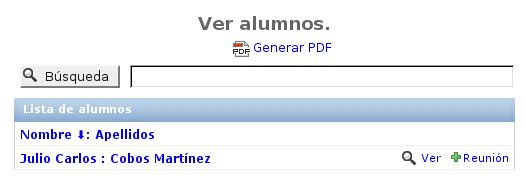
\includegraphics[scale=0.55]{5.Ejemplos_Practicos/5.4.Asesor/ver_alumnos.png}
      }
      \caption{Lista de \textit{Alumnos} de ejemplo.}
      \label{ejemploVerAlumnos}
    \end{center}
  \end{figure}